\chapter{更加通用的高精度流体仿真方法}
\label{sec:sig23}

我们在上一章中已经描述了应用于视觉动画的LBM方法,但是对于工业应用来说,以上的方法并不能满足要求。其中有几个原因。第一个原因是,第~\ref{sec:siga21} 章所描述的混合方法虽然高效,但以真实世界中的风洞举例,在真实的风洞实验中,物体周围的边界层已经非常薄,远小于网格大小,从而在网格层面假设速度是线性的已经不够精确。第二,在这样的尺度下,我们已经无法单纯地依靠提高分辨率,以解决这一问题,而必须依赖于多分辨率网格,在上一章中的方法并没有涉及相关的处理。第三,对于工业应用,碰撞模型等LBM的核心算法,对结果也有着至关重要的影响,而这一点在上一章中也未有足够的讨论。所以在这一章中我们将介绍一个更加通用的高精度流体仿真方法,并更专注于一些实际工业产品设计与验证等应用。更具体地,我们尝试将现实中工业产品设计中非常常见的风洞实验,通过流体仿真的形式数字化。所以在下文中,我们也可将本章中描述的方法称为基于LBM的虚拟风洞测试系统。这个目标使我们不只局限于边界处理等方法本身,还需要整体的仿真框架配合。从而在本章中,我们将更为整体地描述整个仿真框架。当然同时我们也可以将这一系列方法应用在图形学中,相关的结果将在第~\ref{sec:results} 章中展示。

% Sec 4.1
\section{背景与动机}
\paragraph{风洞与虚拟风洞}
从20世纪早期开始,航空工程师开始使用风洞来测试飞机,之后汽车的设计制造也开始使用类似的技术。虽然汽车行业在早期,并不注重空气动力学的影响,许多汽车的造型都以方正和硬朗为特点,但随着汽车越来越注重经济性,尤其是现在进入电动汽车的时代后,空气动力学对汽车造型的设计影响越来越显著。随后更多的领域开始使用风洞测试进行空气动力学特性的测试,如高层建筑物、高速列车、船舰等的设计。虽然风洞实验对产品设计有着很强的指导意义,但是真实的风洞实验需要进行实际的物理建模,并且风洞本身的造价也十分高昂。这样的高成本与操作难度,使其难以被频繁应用。在计算机得以发展后,虚拟风洞随即出现,并成为一种更简单、高效、节约成本的气动设计解决方案。同时虚拟风洞可以更直观地提供可视化结果,如表面的高压与低压区分布、不同位置的气流的涡流程度等。这些数据可以在设计的迭代中节约大量的时间与经济成本。直到今天,虚拟风洞的效率依然深刻影响汽车、建筑、航空航天等领域的产品研发周期~\cite{HighriseBuildings,windScience}。

\paragraph{虚拟风洞的现状}
对于最常见的亚声速弱可压情况 (马赫数小于0.3时,此时流体依然可以用不可压模型进行近似描述),目前的虚拟风洞测试需要经过一个非常耗时的前处理阶段。最耗时的部分是基于物体模型构建贴体的计算网格,这一过程需要大量的人工调整,以保证网格质量。构建好计算网格后,一般使用基于有限体积或有限元的CFD求解器,来求解流体。这样的流体求解即使在CPU集群上,也可能需要数天才可完成一次仿真。在GPU平台上,使用现有软件,如西门子StarCCM+~\cite{Siemens} 进行瞬态流求解,也是类似的效率。所以更多时候,在现有的虚拟风洞实验中会进行稳态求解,以节省计算时间。

\paragraph{使用LBM进行气动分析}
近些年来,LBM在进行高效湍流仿真上,已经取得了长足的进步。LBM在核心算法上的进展已经使其有能力在大规模并行结构上高效求解流体,并达到满足工业应用的精度范围~\cite{Li-2020,Lallemand:2021}。这使得LBM开始在CFD领域成为传统方法之外的一个新的选项 (我们注意到现有的工业软件,如PowerFLOW与XFlow~\cite{Simulia}均基于LBM开发,但其具体使用的方法模型并不明确)。在CG领域,虽然有LBM方法得到了较好的视觉结果~\cite{Li-2020},但其精度依然远比不上工业应用所需的精度。

\paragraph{我们的工作}
我们尝试通过解决一些LBM中的关键问题,提升LBM的整体能力,使得LBM可以成为一个统一的流体仿真框架,以应用到视觉特效、工业设计等多个领域。通过提升碰撞模型、边界处理的精度,结合多分辨率网格与GPU优化,我们构建了一个虚拟的亚声速弱可压风洞测试系统。该系统可以拥有与现有的CFD商业软件相似、甚至更高的精度与计算效率。

% Sec 4.2
\section{方法}
我们的系统相比于现有的LBM主要包含以下四个方面的改进:
\begin{itemize}
	\item 我们对累积量碰撞模型,通过局部熵值的最大化的原则进行了改进。改进后的碰撞模型在精度上有所提升,并可在$10^8$级别的雷诺数下保持稳定; 
	\item 我们提出了一个新的单点插值反弹边界来处理静态与动态物体边界,可以更精准地求解边界层流场;
	\item 我们提出了一个多分辨率网格构建算法,以自动且灵活地构建多分辨率网格,可以在不需花费过多人工前处理的情况下,完成高分辨率流体仿真;
	\item 我们还提出了一系列的GPU优化,进一步提升运算效率。
\end{itemize}

我们将在下面依次介绍这四部分内容。

\subsection{累积量碰撞模型的高阶松弛系数优化}
在碰撞过程中,高阶松弛系数对仿真 (尤其是湍流仿真) 有着很大的影响。Li等~(\citeyear{Li-2020}) 讨论了在中心矩碰撞方法中,进行高阶松弛系数优化的方法。作者通过回归方法,自适应地调整参数,降低了数值色散和耗散误差,提高了数值精度。于是我们希望同样将高阶松弛系数的优化引入累积量碰撞模型中。由于累积量模型的空间变换是非线性的,我们无法直接应用Li等~(\citeyear{Li-2020}) 中的回归方法,或Kramer等~(\citeyear{Kramer-2019}) 中的熵优化方法。但是,我们可以通过一定的推导,将Kramer等~(\citeyear{Kramer-2019}) 中的熵优化方法推广至累积量碰撞模型中。下面我们介绍推导过程。

首先,我们先介绍熵优化的基本思想。分布函数的平衡态$f^\text{eq}_i$可以使熵函数$H(f_i)$取得最大值 (在密度、动量保持不变的前提下)。该熵函数$H(f_i)$定义为
\begin{equation}
\label{eq:entropy_func}
H(f_i)=-\sum_i f_i \log \left(\frac{f_i}{\omega_i}\right) \;,
\end{equation}
其中$\omega_i$是网格权重。所以,可以期待的是,使$H(f_i)$最大化可以使分布函数趋于稳定。这些在Kr{\"a}mer等~(\citeyear{Kramer-2019}) 中有所讨论。
为了优化过程更易求解,我们使用一个二次凹函数$\tilde{H}$对$H$进行近似。$\tilde{H}$称为伪熵 (pseudo-entropy) 函数~\cite{Kramer-2019},表达式为
\begin{equation}
\label{eq:pseudoentropy_func}
\tilde{H}(\bm{f})=-\sum_{i}\left(\frac{f_i^2}{\omega_i}-f_i\right)=\rho-\sum_{i} \frac{f_i^2}{\omega_i}\;.
\end{equation}
该式为$H(\bm{f})$在全局平衡态$f_i^{\mathrm{eq}}(\rho=1, \mathbf{u}=0)=\omega_i$处的泰勒展开。

我们回顾,在分布函数$\bm{f}\!=\!\{f_i\}$与中心矩$\bm{m}\!=\!\{m_i\}$之间存在线性变换关系:$\bm{f}\!=\!\bm{T}\bm{m}$。但与中心矩变换不同,累积量变换是非线性的,所以在累积量碰撞模型中应用熵优化依然是非常复杂的。不过我们通过仔细观察后,可以发现在中心矩$m_{\alpha\beta\gamma}$与累积量$k_{\alpha\beta\gamma}$之间有着关键的联系:当阶数$p\!\leq\!3$时,累积量与中心矩是完全相等的,而高阶累积量是对应的中心矩以及其它中心矩的和 (见第~\ref{sec:cumulant} 节)。由于0-2阶的累积量在碰撞过程中需要根据物理规律来确定松弛系数,3阶累积量的松弛系数在~(\cite{Geier-2017} 中已有过优化方法,我们可以基于此推导使熵最大化的高阶累积量松弛系数的\emph{解析解}。

我们用$\bm{k}_l=\{k_l, l\!\in\!\mathcal{L}\}$表示3阶及以下的累积量,如上述,这些累积量的松弛系数是已知的。
接下来我们可以将剩余的累积量,即4到6阶的,表示为$\bm{k}=\{k_h, h\!\in\!\mathcal{H}\}$。那么,伪熵的最大化问题可以被写作
\begin{equation}
    \label{eq:entropy_opt_problem}
    \bm{f}^{*} = \underset{\bm{k}}{\arg \max } \tilde{H}(\bm{f}).
\end{equation}
我们将中心矩$m_i$与对应的累积量$k_i$之间的差定义为$r_i$:
\begin{equation}
    r_i = m_i - k_i.
\end{equation}
那么$f_i$可被相应写作:
\begin{align}
    f_i &= \sum_{l \in \mathcal{L}} t_{il}m_l+\sum_{h \in \mathcal{H}} t_{ih}m_h \\
    &= \sum_{l \in \mathcal{L}} t_{il}(k_l + r_l)+\sum_{h \in \mathcal{H}} t_{ih}(k_h + r_h).
\end{align}
其中$t_{ij}$是$\bm{T}$的元素,即$\bm{T}=\{t_{ij}\}$。
由于累积量和中心矩在三阶及三阶前是相等的,所以有$r_l = 0, l \!\in\! \mathcal{L}$,使得
\begin{align}
    f_i &= \sum_{l \in \mathcal{L}} t_{il}k_l + \sum_{h \in \mathcal{H}} t_{ih}(k_h + r_h). \label{eq:fi_as_cumulants}
\end{align}
对于公式~\ref{eq:entropy_opt_problem} 所描述的问题,我们可以对下式求解来得到$k_h$:
\begin{equation}
    \label{eq:entropy_opt_derivative}
    \frac{\partial \tilde{H}(\bm{f})}{\partial k_h} = 0, h \in \mathcal{H}.
\end{equation}
公式~\ref{eq:entropy_opt_derivative} 的左手侧可以被展开写作
\begin{equation}
    \frac{\partial \tilde{H}(\bm{f})}{\partial k_h} = -\sum_i \frac{\partial f_i}{\partial k_h} \cdot \frac{2 f_i}{\omega_i}.
\end{equation}
将公式~\ref{eq:fi_as_cumulants} 代入公式~\ref{eq:entropy_opt_derivative},则公式~\ref{eq:entropy_opt_derivative} 可以被重新写作
\begin{equation}
    \label{eq:entropy_opt_expanded}
    \sum_i \frac{\partial f_i}{\partial k_h} \cdot \frac{\sum_{h \in \mathcal{H}} t_{ih}(k_h + r_h)}{\omega_i} = -\sum_i \frac{\partial f_i}{\partial k_h} \cdot \frac{\sum_{l \in \mathcal{L}} t_{il}(k_l + r_l)}{\omega_i},
\end{equation}
现在,如果我们定义$\bm{r} = \{r_h, h \!\in\! \mathcal{H}\}$,一个重要的发现是,存在一个可以用解析式表达的矩阵$\bm{\underline{L}}$使得
\begin{equation}
    \bm{r} = \bm{\underline{L}} \,\bm{k}_h \,+\,  \bm{\underline{n}}\;, \label{linearRelationKvsM}
\end{equation}
并且$\bm{\underline{L}}$中不含未知量。公式~\ref{linearRelationKvsM} 中的$\bm{\underline{n}}$也只含有已知的低阶累积量,所以$\bm{r}$与$\bm{k}_h$本质上成线性关系。
我们将矩阵$\bm{T}$分解为$\bm{T} = [\bm{T}_l; \bm{T}_h]$,定义$\bm{D} = [\frac{\partial f_i}{\partial k_h}] = \bm{T}_h(\bm{I} + \bm{\underline{L}})$,并将单位矩阵记作$\bm{I}$,$\omega_i$组成的对角矩阵记为$\bm{W}$,则公式~\ref{eq:entropy_opt_expanded} 可以用矩阵的形式描述为
\begin{equation}
    \bm{D}^T \bm{W}^{-1} \bm{T}_h ((\bm{I} + \bm{\underline{L}}) \bm{k}_h + \bm{\underline{n}}) = -\bm{D}^T \bm{W}^{-1} \bm{T}_l \bm{k}_l .
\end{equation}
经过变换后,可得到$\bm{k}_h$的表达式
\begin{equation} \label{eq:solution}
	(\bm{I} + \bm{\underline{L}}) \bm{k}_h =  -(\bm{D}^T \bm{W}^{-1} \bm{T}_\text{h})^{-1}\bm{D}^T \bm{W}^{-1} \bm{T}_\text{l} \bm{k}_\text{l} - \bm{\underline{n}} \;.
\end{equation}
至此,我们得到了D3Q27网格结构下,通过熵优化进行累积量碰撞模式进行高阶松弛系数优化的方法。该方法可以通过一个简单的线性求解得到$\bm{k}_h$,并且由于有解析解的存在,在求解的过程中并没有过高的计算代价。为了避免数值偏移,优化后的累积量要被限制于平衡态和碰撞前的数值之间。剩余的碰撞过程与第~\ref{sec:cumulant} 节中的描述一致。

\subsection{单点插值反弹边界处理}
\paragraph{静态边界处理}
\begin{figure}[htb]
  \centering
    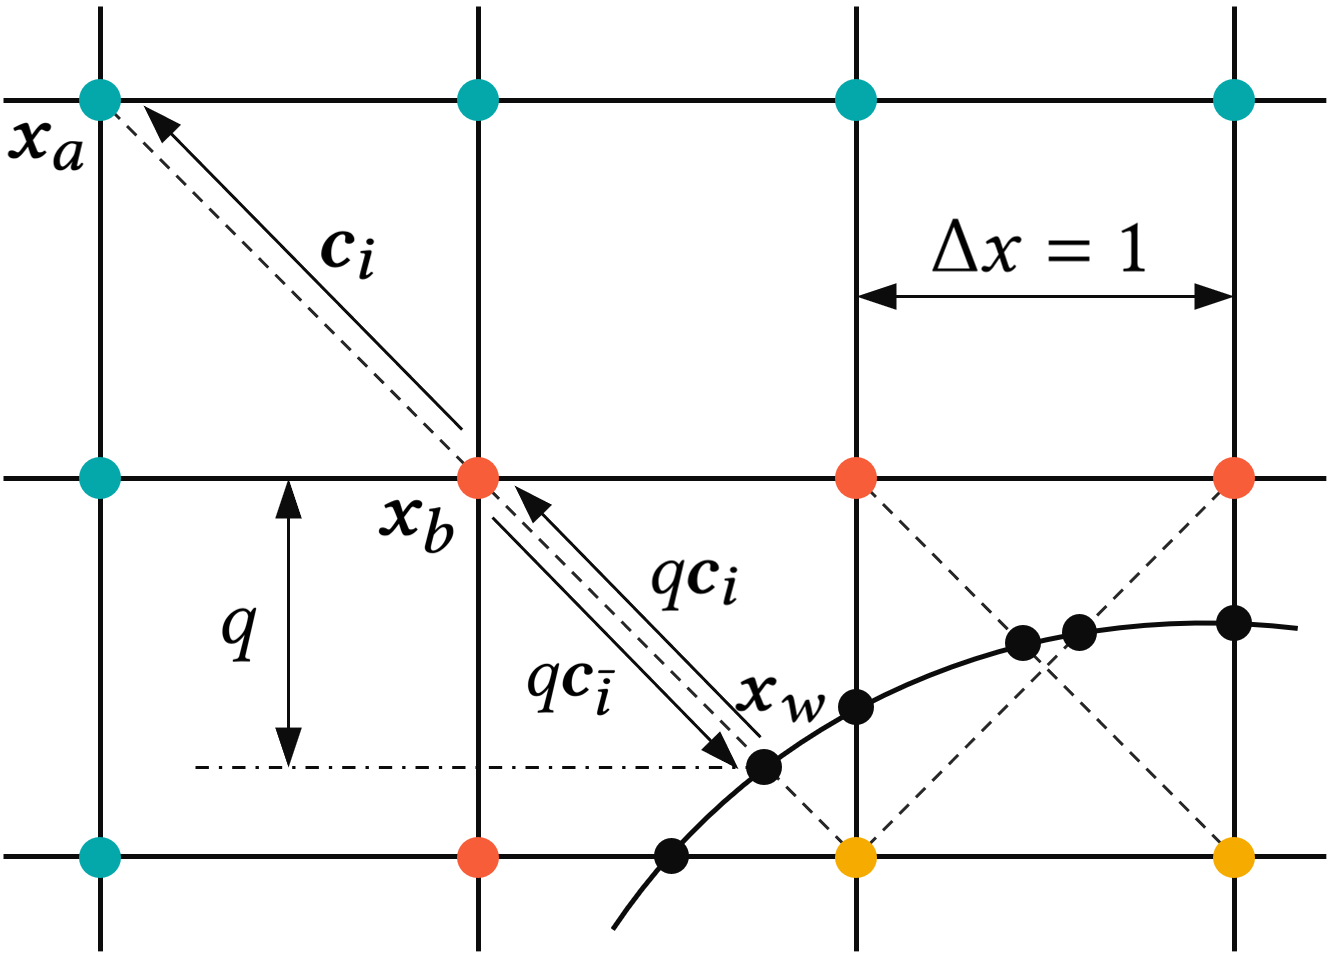
\includegraphics[width=0.6\columnwidth]{figures/boundary.png}
  \bicaption[固体附近的边界处理]{固体附近的边界处理。对于切削网格点 (图中标为橘色),它们的未知分布函数必须要通过边界处理决定。图中黄色点为固体内部点,青色点为流体点。对于$\bm{x}_b$点,$q$表达该点沿$\bm{c}_i$方向到边界的归一化距离,其中$\bm{c}_{\bar{i}}$为$\bm{c}_i$的反方向。}{Boundary treatment near solid object. For ``cut-cell'' boundary nodes marked in orange, their unknown distribution functions must be determined through boundary schemes instead of the regular streaming. Yellow nodes mark nodes inside the solid while cyan nodes are fluids nodes. Our boundary treatment for a node $\bm{x}_b$ uses the normalized distance $q$ to the boundary surface along a link direction of $\bm{c}_i$ with its inverse direction denoted as $\bm{c}_{\bar{i}}$.}
  \label{img:boundary}
\end{figure}

\begin{figure}[htb]
	\centering
	  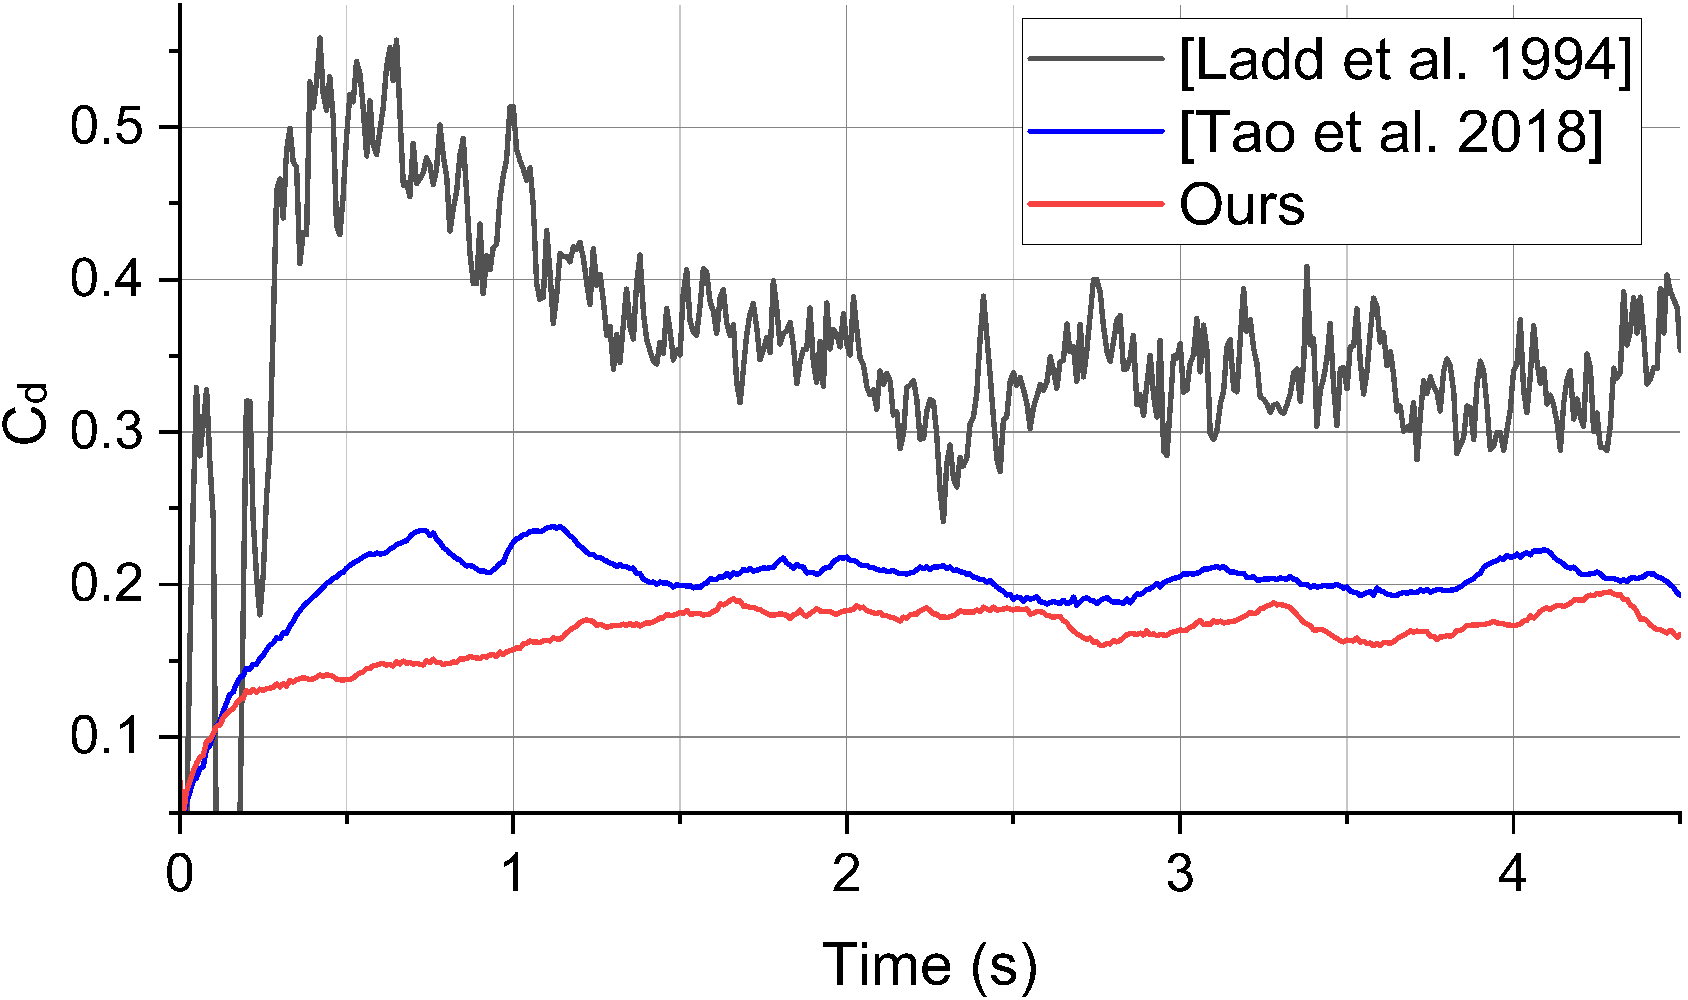
\includegraphics[width=0.7\columnwidth]{figures/bnd_comp.png}
	\bicaption[边界处理的比较]{边界处理的比较。对于$Re=400,000$风吹过球的场景,我们画出了使用不同边界处理进行仿真得到的球的阻力系数。仿真中的碰撞模型均为使用了熵优化的累积量碰撞模型。该场景在实际实验中得到的球的阻力系数$C_\text{d}\!=\!0.1$。虽然简单反弹边界依然在许多LBM中得到应用,但是其结果误差及波动均过大,无法得到可置信的结果。}{Comparing boundary treatments. We plot the variation over time of drag coefficient of a sphere at $Re=400,000$, for different boundary treatments but with the same entropy-optimized cumulant model. The experimental value is near $C_\text{d}\!=\!0.1$ for this drag crisis case; a simple bounce-back, still used in many LBM implementations, leads to unacceptable results, producing large prediction errors and wide force fluctuations.}
	\label{img:bnd_comp}
  \end{figure}

在虚拟风洞的绝大多数情况中,目的都是对某个物体进行气动的性能测试。所以在虚拟风洞的应用中,边界处理的重要性是不言而喻的。边界处理的示意图见图~\ref{img:boundary}。其中橘色点为需要进行边界处理的流体点,黄色点为固体内部点。
我们在第~\ref{sec:boundary_treatment} 节中已经讨论了简单反弹边界和插值反弹边界的形式。其中简单反弹边界虽然构造形式非常简单,但是在边界形状复杂时,一般只有一阶精度。从而在计算固体受力时,误差及波动是非常剧烈的 (见图~\ref{img:bnd_comp} 中展示的风在高雷诺数下吹过球时,球的阻力系数$C_\text{d}$变化)。
插值反弹边界~\cite{Bouzidi-2001} 与其之后的变体~\cite{Yu-2003, Ginzburg-2003, Chun-2007} 则可以使边界求解的精度达到二阶或更高。然而,这些边界处理方法均需要相邻点的参与,使得计算不再完全局部。由于GPU并行计算中,不连续数据访问对并行效率有很大影响,这样的边界处理在GPU计算上的效率有所降低。此外,当边界点周围均为边界时,找不到相邻点会使这样的边界处理方法失效。
而最近,Tao等~(\citeyear{Tao-2018-b}) 通过在边界上构造额外的分布函数,提出了一个单点的插值反弹边界方法,克服了这一问题。
具体地,如图~\ref{img:bnd_comp} 中所描绘的,我们用$\bm{x}_{b}$表达固体边界附近需要边界处理的点,$\bm{c}_{i}$为指向$\bm{x}_{a}$的方向,$\bm{c}_{\bar{i}}$为相反的方向并与固体边界相交于$\bm{x}_{w}$。跟随之前的插值反弹边界方法中的假设,我们认为这之中存在线性关系:
\begin{equation}
f_i(\bm{x}_b, t\!+\!1) = \frac{1}{1+q}f_{i}(\bm{x}_w, t\!+\!1)+ \frac{q}{1+q}f_{i}(\bm{x}_a, t\!+\!1) \;,
\end{equation}
其中$q=\|\bm{x}_b - \bm{x}_w\|/\|\bm{c}_i\|$是边界点到边界的归一化距离。
因为分布函数$f_{i}(\bm{x}_a, t+1)$可以从$\bm{x}_b$的前一时刻迁移过来,所以这里的线性插值实际上只涉及一个点的数据。
而边界上的未知分布函数$f_{i}(\bm{x}_w, t\!+\!1)$可以由平衡态$f_{i}^\text{eq}(\bm{u}_w(t), \rho_b(t))$与b点的非平衡态$f_{i}^\text{neq}(\bm{x}_b, t)$相加得到,其中$\bm{u}_w(t)$为边界点的速度。$f_{i}^\text{neq}(\bm{x}_b, t)$可以表达为
\begin{equation}
f_{i}^\text{neq}(\bm{x}_b, t) = f_{i}(\bm{x}_b, t) - f_{i}^\text{eq}(\bm{u}_b, t).
\end{equation}
然而由于这样的构造使用了低阶的泰勒展开近似,在高雷诺数仿真中精度并不足够。为了进一步提升精度,我们提出一种新的构造平衡态和非平衡态的方法。
首先,我们可以利用非平衡态的阶数比平衡态高一阶的性质~\cite{Chun-2007},意味着我们可以对$\bm{x}_b$点的非平衡态进行简单反弹,而并不会影响整体解的精度。用公式表达为
\begin{equation}
\label{eq:neq_bb}
f^\text{neq}_{i}(\bm{x}_b, t\!+\!1) = f^\text{neq}_{\bar{i}}(\bm{x}_b, t).
\end{equation}
对于平衡态部分,我们可以采用与~\cite{Tao-2018-b} 同样的二阶精度单点插值方法
\begin{align}
f^\text{eq}_i(\bm{x}_b, t\!+\!1) &= \frac{1}{1+q}f^\text{eq}_{i}(\bm{x}_w, t\!+\!1) + \frac{q}{1+q}f^\text{eq}_{i}(\bm{x}_a, t\!+\!1).
\end{align}
虽然$f^\text{eq}_{i}(\bm{x}_w, t\!+\!1)$可以由$f_{i}^\text{eq}(\bm{u}_w(t), \rho_b(t))$近似,但我们仍然需要确定如何求得$f^\text{eq}_{i}(\bm{x}_a, t\!+\!1)$。
由于我们无法获得$t+1$时刻的宏观量,一种方法是通过宏观量$\bm{u}(\bm{x}_a, t)$与$\rho(\bm{x}_a, t)$来重建平衡态。这样的做法相当于将平衡态公式对$t$进行泰勒展开后,进行了0阶逼近。这样的逼近势必在高雷诺数仿真中对边界层附近有负面的影响。
所以,我们利用$f^\text{eq}_{i}(\bm{x}_a, t\!+\!1) \approx f_{i}(\bm{x}_a, t\!+\!1)$来进行逼近,以不进行任何截断。并且$f_{i}(\bm{x}_a, t\!+\!1)$可以直接从$\bm{x}_b$迁移获得。所以我们得到
\begin{equation}
\label{eq:eq_a}
f^\text{eq}_{i}(\bm{x}_a, t\!+\!1) \approx f^{*}_{i}(\bm{x}_b, t).
\end{equation}
结合公式~\ref{eq:neq_bb} 与公式~\ref{eq:eq_a},未知分布函数$f_i(\bm{x}_b, t\!+\!1)$可以被写为
\begin{align}
f_i(\bm{x}_b, t\!+\!1) &= f^\text{eq}_i(\bm{x}_b, t\!+\!1) + f^\text{neq}_{i}(\bm{x}_b, t\!+\!1) \\
&= \frac{1}{1\!+\!q}f_{i}^\text{eq}(\bm{u}_w(t), \rho_b(t)) + \frac{q}{1\!+\!q}f^{*}_{i}(\bm{x}_b, t) + f^\text{neq}_{\bar{\imath}}(\bm{x}_b, t).\nonumber
\end{align}

\paragraph{动态耦合}
虚拟风洞中也需要一部分动态的单向耦合,如汽车仿真时轮胎的旋转。
之前的LBM通常结合格点重填与反弹边界条件~\cite{Tao-2016},或使用浸没边界法~\cite{Li-2016, Li-2020}进行动态耦合。
但格点重填结合反弹边界条件的方法在高雷诺数仿真中会在边界周围产生不正常的速度。而浸没边界法虽然更容易实现,但因为只有一阶精度,则达到同样精度需要更高的分辨率进行仿真,从而消耗更多的资源。
为了保证在薄边界层上保证更高的精度,在动态耦合时,我们依然应用上述的静态边界处理方法,不同点是现在各个切削速度方向的$\bm{u}_w$都需要求解。为了避免格点重填,我们依然使用浸没的模式来处理边界,即所有的格点我们都认为是流体点,没有固体点。当然我们注意到,要在每个时间步都进行求交并求解边界的速度,通常需要进行层级搜索~\cite{Karras-2012},而当分辨率非常高时,在GPU上进行这样的操作非常耗时。
于是我们提出了相应的GPU实现,以减轻求交与动态耦合的计算开销。这些算法我们在第~\ref{sec:sig23_alg_optimal} 节中介绍。

\paragraph{计算域边界处理}
在固体边界之外,还有一些边界也需要进行处理,其中一类就是计算域边界。计算域的边界同样对仿真得到的物理量有很大影响。我们在实现时使用了滑移边界条件 (slipping boundary conditions) 来处理入口与出口之外的计算域边界。虽然有多种方法可以实现滑移边界~\cite{Kruger-2016},但这些方法的精度不足以在强湍流中准确求解计算域边界处的流体,并会对物体附近的流体产生影响。于是我们需要扩大计算域来减轻其影响,但这样会额外增加仿真的时间和存储成本。
为了弥补这一问题,我们在计算域边界首先采用$\bm{u}_w \!=\! \bm{u}_n$的边界条件,其中$\bm{u}_n$是沿着计算域边界法向方向,距边界最近的流体点的速度。
然后使用这一边界速度,我们将计算域边界视为动态边界并使用上述方法进行处理。同样的处理也可以应用在计算域的入口或出口上。在已知速度或压力后,未知的分布函数可用同样的边界处理方法获得。我们通过这样的处理,避免计算域边界对计算域内部产生过大的影响。

\paragraph{地面处理}
由于虚拟风洞中的实验经常要与现实风洞实验相对应,很多时候模型会被放置在地面上。此时由于地面与模型距离非常接近,地面的边界处理对精度有着非常大的影响。所以在模型被放置在地面时,我们不能认为地面是普通的计算域边界,而要进行特殊处理。我们这里的特殊处理方法使用了壁面函数~\cite{Malaspinas-2014},即通过地面上方的格点与壁面函数,推导出地面速度$\bm{u}_g$。而地面的密度可以认为与地面上方的点一致 (即诺伊曼边界条件$\nabla \rho \cdot \bm{n} \!=\! 0$)。具体的宏观量推导过程由于篇幅限制,无法按步骤详细列出,请读者参见~\cite{Malaspinas-2014}。
在获得地面的宏观量之后,我们重建未知的分布函数$\smash{f_i \!=\! f_i^{eq} + f_i^{neq}}$,其中
\begin{align} 
    f_i^{eq} &\approx w_i \rho_g+\biggl(1+\frac{\bm{c}_i \cdot \bm{u}_g}{c_s^2}+\frac{\left(\bm{c}_i \cdot \bm{u}_g\right)^2}{2 c_s^4}-\frac{\bm{u}_g \cdot \bm{u}_g}{2 c_s^2}\biggr), \\
    f_i^{neq} &\approx -\frac{\tau \rho_g \omega_i}{2 c_s^2} \langle \bm{Q},  \nabla \bm{u}_g + \nabla \bm{u}_g ^ T \rangle,\\[-6mm]\nonumber
\end{align}
这里面$\smash{Q_{\alpha\beta} = c_{i\alpha} c_{i\beta} - c_s^2\delta_{\alpha\beta}}$ ($\delta_{\alpha\beta}$是克罗内克 (Kronecker) $\delta$函数)。
使用这样的壁面函数处理地面,在高雷诺数流体仿真中,依然不足以获得足够高精度的解。原因是地面可能与模型本身形成一条窄缝 (想象汽车在地面上时,底盘与地面之中的间隙),在这种情况下流体的运动情况很难被现有的LBM准确捕捉。我们注意到类似情况的边界处理仍然是热门的研究课题,所以在这一方向若有后续工作可以对地面处理部分进行改进。

\paragraph{固体受力计算}
对于上述的边界处理,我们依然可以用动量交换法计算固体受力~\cite{Ladd-1994, Mei-2002},即对于边界点$\bm{x}$有
\begin{equation}
    \Delta \bm{p}(\bm{x})= \sum_{j\in L(\bm{x})} \bm{c}_{j'}\,(f_{j}(\bm{x}) + f^*_{j'}(\bm{x})),\vspace*{-1.5mm}
\end{equation}
其中$L(\bm{x})$为$\bm{x}$点向外的速度方向 (由固体向流体方向),$f_{j}(\bm{x})$为通过边界处理方法得到的分布函数。则固体受到的合力为所有边界点上受力的和
\begin{equation}
    \bm{F} = \sum_{\bm{x}} \Delta \bm{p}(\bm{x}).\vspace*{-1mm}
\end{equation}
注意因为我们使用了浸没的思想,所以所有的切削网格点都应被视为边界点。

\subsection{多分辨率仿真}
\label{sec:multi-res}
如果我们在单分辨率网格上应用上述的算法,对于图形学领域的应用应该足够。因为一般图形学中的物体模型较为简单,且我们只需捕捉视觉现象。但应用于工程领域,虚拟风洞需要被应用至非常大的场景 (一般对于4m左右长度的汽车模型需要40m$\times$20m$\times$20m的计算域),且几何模型的精度需要有3mm或更高的解析度,以捕捉到足够小的流体特征。这些特征也许对湍流本身的视觉效果来说没有明显改变,但是它们对物理量的大小有关键的影响。使用单分辨率网格进行这样高分辨率的仿真无论从仿真时间或内存和显存的占用考虑,都是不切实际的。所以显然多分辨率网格在工业领域流体仿真应用中是不可或缺的~\cite{Hou-2019,Aultman-2022,Romani-2022}。

然而,我们已经讨论过,许多传统的基于有限体积法的N-S求解器均需要非结构化网格。对于工业精度的几何模型,构建这样的网格是十分耗时的。虽然针对非结构化网格,有自动化的网格构建方法,但是由于模型的高复杂性,网格中产生空洞或尖角的情况依然无法避免,这些会导致FVM的求解最后无法收敛。而对模型的检查、修复需要专业工程师的人工努力,这对实际工业设计中的工作效率有很大影响。

在LBM的文献中,多分辨率网格方法一般都基于八叉树的数据结构~\cite{EitelAmor-2013,Hasert-2014},但是要在GPU上完成高效且可扩展的实现是十分复杂的~\cite{Schornbaum-2016, Schornbaum-2018}。而我们提出了新的全自动网格构建算法,以支持十分复杂的几何模型与更简单、高效的GPU实现。下面我们描述该算法的具体过程。

\paragraph{多分辨率网格构建}
自动的网格细化一般都需要基于一定的标准来指导对哪一部分进行细化。这其中最常被考虑的应该是来流方向及网格到边界的距离~\cite{Sandoval-2012,Li-2019}。
于是我们也主要围绕这两个因素,设计我们的自动网格构建方法。
对于一个模型,我们首先将该模型的轴对齐包围盒 (axis-aligned bounding box, AABB) 的每个维度延长一定的距离$d^*$,这个距离表示贴体网格的厚度。至此我们得到了一个比模型稍大的方形区域$\Omega_n$ (见图~\ref{img:grid_construction} 中的红色方框区域)。为了方便网格间的数据过渡,从粗到细,每层格子间的网格大小均是上一层的2分之1。同时格子间要有部分的重叠以减小网格数据过渡的误差。
下面我们将整个计算域标记为$\Omega$,并将纯流体区域标记为$\Omega_f \!=\! \Omega \setminus \Omega_n$。在$\Omega_f$中,我们主要考虑来流方向。
即$\Omega_f$中的所有网格均会沿来流方向延伸,以用更细的网格覆盖物体后的尾流部分 (见图~\ref{img:grid_construction} 中从蓝色到黄色的网格)。
而在$\Omega_n$中,我们对每一个点计算一个到模型的距离,构成一个无符号距离场 (我们会在下面讨论为什么不使用有符号距离场),之后保留所有距离小于$d^*$的点 (见图~\ref{img:grid_construction} 中的橘色网格)。在计算距离场时,我们使用了Imre等~(\citeyear{Imre-2017}) 提出的高效GPU距离场计算方法。通过这样我们得到的多分辨率网格并不需要树形结构进行组织,同时也可以使各层网格间顺利地进行数据过渡,而避免Li等~(\citeyear{Li-2019}) 所提出的连续尺度方法中大量的内存及显存消耗。

\paragraph{针对动态物体构建网格}
为了应用于虚拟风洞测试,我们必须考虑一定的动态物体。由于风洞中需要双向耦合的频率远低于单向耦合,所以这里我们只考虑单向耦合。依然从该物体的AABB出发,我们将该模型所有可能经过的位置都设为最细的网格区,以满足边界附近的精度。这样的构建对如轮胎旋转等物体绕轴旋转的场景十分适合,因为物体的运动几乎不会扩大网格覆盖的范围。但是对于更复杂的运动,如飞机的起落架从机腹中落下这样的场景,虽然可以使用同样的方法构建网格,但会浪费大量的细网格,从而造成显存浪费。我们认为这一部分可以在未来工作中有所改进。

\begin{figure}[htb]
	\centering
	  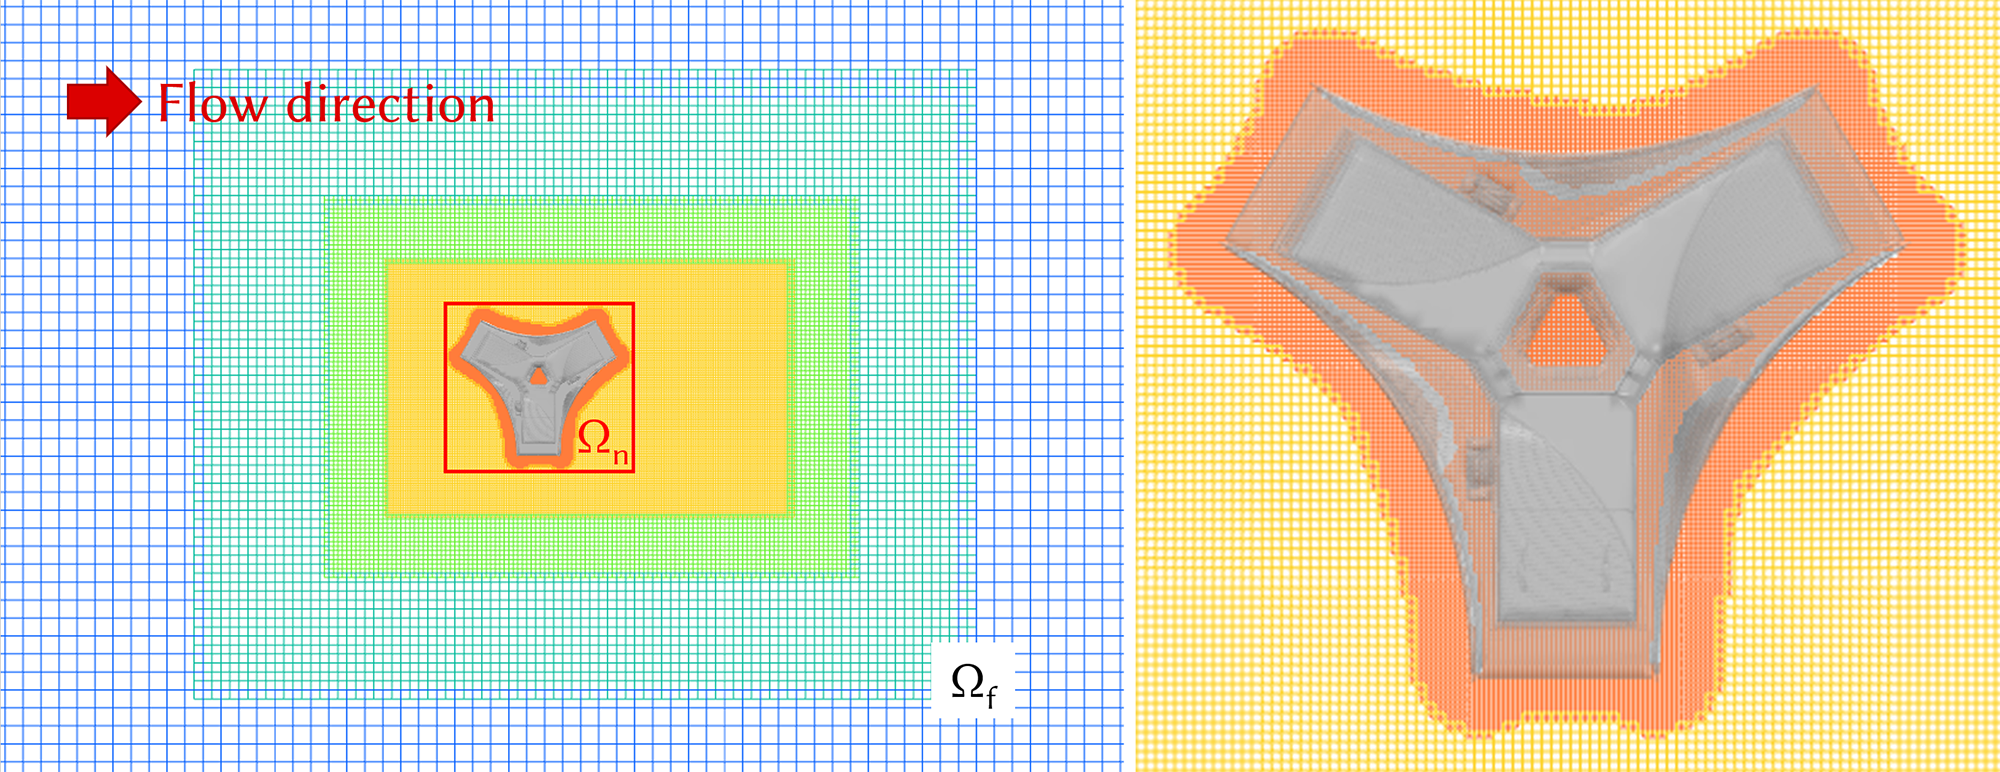
\includegraphics[width=0.9\columnwidth]{figures/grid_construction.png}
	\bicaption[多分辨率网格的构建]{多分辨率网格的构建。为了尽可能在节约内存与显存使用的同时,依旧维持足够的仿真精度,我们依据来流方向对所有网格进行自动构建 (最后一层网格除外,见左图)。即除最后一层网格外,每一层网格均有一定的方向性扩展。这个扩展是为了更准确的捕捉建筑物模型后的尾流。最后一层网格依据到边界的距离进行构建。最后我们通过传播找到所有的有效流体点,以保证场景中每一个连通部分都可以参与流体计算 (前提是这些连接部分至少大于最细网格的大小,见右图)。}{Multiresolution grid construction. To keep memory size low when computing accurate predictions of physical quantities, multiresolution grids are automatically constructed, with a refinement guided by the incoming flow direction for all but the last grid level (left) --- explaining the offset of the different levels of grid compared to this architectural building so as to capture its wake accurately --- then by the distance to the object. All active fluid nodes are finally found by flooding to ensure that the flow goes through all the mesh openings larger than the finest grid resolution (right).}
	\label{img:grid_construction}
  \end{figure}

\paragraph{针对复杂物体构建网格}
如果我们认为物体模型至少是闭合的,那么我们通过有符号距离场 (signed distance field) 已经可以有效地分辨格点位于物体的内外。但是在实际应用中,很多模型并不具有这样的良好特质。如汽车的栅格实际上可以视作汽车内部的空气入口,建筑模型也有很多很小的开口足以使空气流入。
在这种情况下,我们无法实际判别物体内外。所以我们在最细的网格上使用一个传播算法,来标记所有有效的网格点。具体地说,我们从一个已知的流体点出发,如$\Omega_n$中的网格原点,沿各个速度方向检查该点与其邻居是否相连。相连的标准为它们之间的速度方向是否与物体边界相交,若相交则认为不连通。该过程的一个二维示例见图~\ref{img:propagation}。
我们将所有连通的点标记为有效流体点后,继续重复这一过程,进行广度优先搜索,以找到所有的有效流体点。
这样做的好处主要有两个。第一个为我们可以剔除掉所有的固体点,因为固体点对仿真没有实际影响。这样我们可以进一步节省显存占用。第二个为我们可以同时将边界处理时所需要的归一化距离$q$一并求出,留至之后边界处理时使用。

\paragraph{网格间数据过渡}
接下来我们必须考虑数据如何在不同网格大小的网格间传递、过渡。这一方面我们使用了~\cite{Lagrava-2012} 中提出的方法。该过程可简要概括如下。对于两个网格之间的数据交互,永远存在一个较粗的网格和较细的网格 (两个网格的网格大小是2倍关系),并且这两个网格中会有一定的重叠区域以方便过渡 (这些在我们的网格构建方法中已经通过约束保证)。那么粗、细网格会交替执行仿真。由于网格大小的2倍关系,为了保证同样的黏度,它们的时间步长也是2倍关系,即粗网格仿真一个时间步长,细网格需仿真两个时间步长。在这两个网格中,最外层的格点均可视为需要进行网格过渡的格点 (我们接下来称为待求点),因为它们的分布函数信息无法靠自己获得,只能从另一网格获得。而因为重叠区域的存在,细网格的待求点在粗网格中是正常格点。同理,粗网格的待求点在细网格中也是正常格点。所以,在两个网格交替前进时间步长的过程中,待求点的信息都可以从另一个网格插值得到。而这个插值需要分为平衡态与非平衡态。因为平衡态部分只取决于宏观量,而宏观量在不同网格中是不变的。但非平衡态部分与应力张量有关,在不同网格间有一定的比例关系,所以在不同网格间插值时需要进行缩放。关于整体数据过渡的细节可参考~\cite{Lagrava-2012}。
这一过程其实对于每一对 (粗、细) 网格都是相同的,所以可以从粗到细以递归的方式完成。
% Fig.~\ref{img:vis_building} for instance shows an instantaneous macroscopic velocity field cross-section from the simulation of the same architecture model from Fig.~\ref{img:grid_construction} using this interpolation approach.

\begin{figure}[htb]
    \centering
      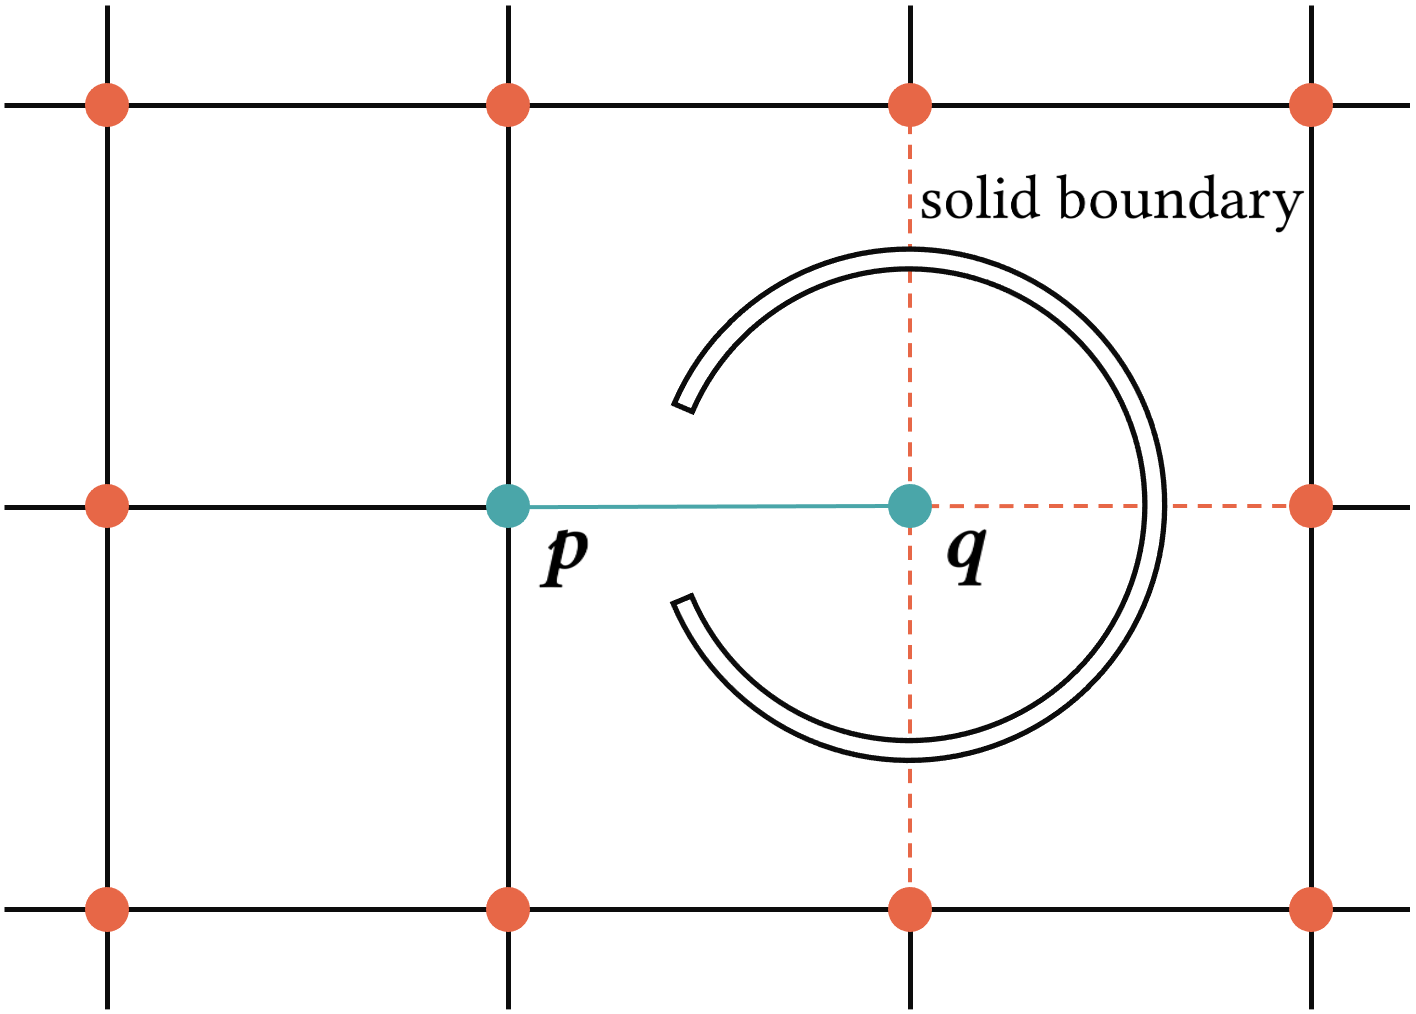
\includegraphics[width=0.7\columnwidth]{figures/propagation.png}
    \bicaption[通过传播找到有效的流体点]{通过传播找到有效的流体点。为了找到并标记所有有效的流体点,我们从一个已知的流体点出发 (如图中的$\bm{p}$点),然后我们找到该点所有的邻接点,检测它们之间的连接有没有与固体边界相交。如果两点间的连接没有与边界相交 (如$\bm{p}\bm{q}$),则点$\bm{q}$被标记为新的有效流体点。这个过程以广度优先顺序重复,直到找到所有有效的流体点,使所有的连通部分相互连接}{Propagation of valid fluid nodes. To find and tag all valid fluid nodes, we start from an already known fluid node, e.g., node $\bm{p}$ in 2D, then we check its immediate neighbors to see whether a link intersects a boundary. If no intersection is detected (e.g., link $\bm{p}\bm{q}$), the untagged node $\bm{q}$ is tagged as a new valid fluid node. This process repeats in a bread-first search order, enabling internal regions to be connected to the external fluid region.}
    \label{img:propagation}
\end{figure}

\section{算法优化}
\label{sec:sig23_alg_optimal}
我们接下来讨论一些我们在实现过程中发现的,对计算效率有重要影响的方面,及我们的优化方法。
% An overview of our simulation process is summarized in Alg.~\ref{alg:simulation}.

\paragraph{高效链路-几何求交}
在边界处理中,每一步我们都需要得到边界点上各链路到几何模型的距离。对于静止模型,我们可以只在前处理中做一次求交,但是对动态物体,由于其形状在不停改变,我们需要在每个时间步都进行一次求交。由于求交的复杂性,这一步在时间上的消耗甚至大于仿真本身的消耗。
为了解决这一问题,我们采用与浸没边界法~\cite{Chen-2021}中的扩散 (spreading) 类似的想法,以物体模型的元素为出发点,寻找周围的流体点,而不是以流体点为并行单元进行并行。
对于边界上的每个元素 (在三维中通常为三角形),我们找到所有该元素覆盖的网格。这一步只需不遗漏网格即可,所以使用该元素的AABB也是可以的。这一过程的一个二维示意图可见图~\ref{img:intersection},在二维中模型元素是线段而不是三维中的三角形。
对于每个覆盖的网格,格点上的所有链路都会与该模型元素进行求交测试。如果有链路相交,则我们在这个格点上记录归一化距离$q$,这个距离会在边界处理中被使用。
这样做的优势是,每个模型元素所找到的流体点的数量都是相对较少的,这在GPU上有着数据连续和负载均衡的优势。为了测试效率,我们使用一个4.5 m长的、元素数量在1千万的模型,在一个网格大小为4 mm的计算网格中求交。结果显示使用上述的求交方法,相比传统的树状结构加速的方法,效率的提升在大约十倍。这可以有效地提升整体仿真的计算效率,尤其是场景中有动态物体时。

\begin{figure}[htb]
  \centering
    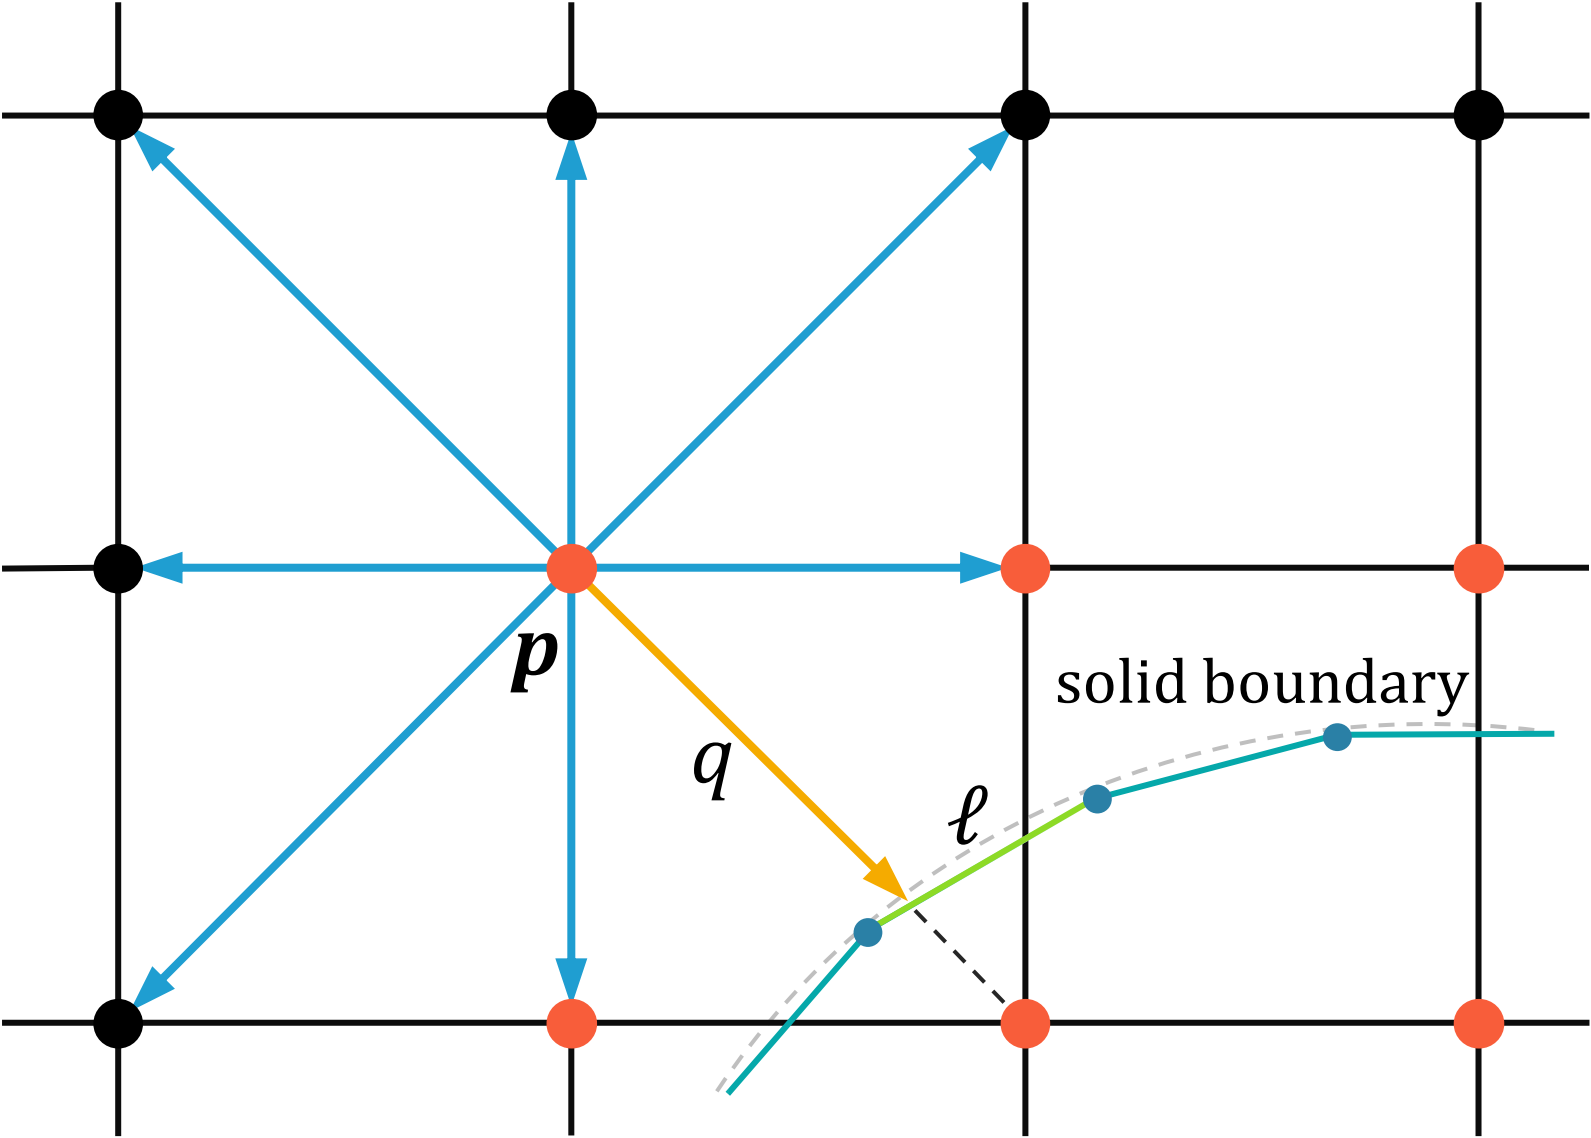
\includegraphics[width=0.7\columnwidth]{figures/intersection.png}
  \bicaption[高效链路-几何求交]{高效链路-几何求交。我们不使用传统方法,即将模型的元素放入一个树形结构中进行查找。我们使用以模型元素作为并行单元,来查找附近和其相交的链路。这里在二维中,模型元素是线段,而三维中一般是三角形。对于一个模型元素,我们可以很快地找到其所覆盖的网格,并于可能相交的链路依次求交。}{Efficient link-boundary intersection. Instead of building a tree-based data structure, we parallelize our link-mesh intersection over all boundary elements --- here boundary edges $\ell$ in 2D. For a given boundary edge, we efficiently locate the cells that the edge straddles, and perform intersection for every link of the nodes that belong to the covered cells.}
  \label{img:intersection}
\end{figure}

\paragraph{数据布局}
在LBM中,分布函数的迁移是必须要访问邻接点的。而GPU中数据的访问顺序又直接影响显存的数据吞吐量,进而影响计算效率。所以设计一定的数据布局以适应LBM的访问对LBM的效率也有很大影响 (尤其是在多分辨率网格中)。
首先整体上,我们依然使用~\cite{Chen-2021} 中的数组结构体结构。一个需要注意的点是,我们构建出的网格中,有效流体点并不一定连续,所以我们需要一个紧凑且GPU友好的数据结构来存储有效流体点的索引。然而在我们的测试中,完美空间哈希 (perfect spatial hashing)~\cite{Lefebvre-2006} 或用于稀疏矩阵的紧凑存储结构~\cite{Greathouse-2014} 表现均不够好。在测试中两者均会增加显存读取频率并使数据访问更不连续,造成计算效率下降。使用针对不规则数据的z-排序 (z-ordering) 结构~\cite{Chen-2021} 也并没有获得预期的性能提升。
所以,为了实现简单,我们生成了一个简单的索引映射 (index map),即以x-y-z顺序,直接在一个线性数组中记录所有流体点的显存索引。这样的数据布局与~\cite{Chen-2021} 中的基于块的存储方法的性能接近,但实现会简单很快。我们认为多分辨率LBM网格的数据布局也是未来可以改进的方向之一。

\section{与现有方法的对比}
\begin{figure}[htb]
  \centering
    \includegraphics[width=0.99\columnwidth]{figures/entropy_comp.png}
  \bicaption[不同累积量模型的对比]{不同累积量模型的对比。我们分别用~\cite{Geier-2017} (图中黑色曲线) 与我们的方法 (图中红色曲线) 对球进行风洞实验,并将$C_\text{d}$随时间的变化画在图中。我们分别在雷诺数Re=100,000 (a)、Re=400,000 (b) 与Re=800,000 (c) 时进行实验,Re=400,000 为球发生阻力危机时的雷诺数。从图中可以看出,我们的方法有着更快的收敛速度与更小的结果波动,使我们方法更适合于计算物体的平均阻力。}{Comparing drag for various cumulant models. We plot drag coefficient $C_\text{d}$ over time for a sphere in a flow using the cumulant model of~\cite{Geier-2017} (black) vs. our entropy-based cumulant model (red) for Re=100,000 (a), Re=400,000 (b) at which drag crisis happens, and Re=800,000 (c) indicating better performance of our model as evidenced by faster convergence and smaller fluctuations --- which both imply a more reliable mean drag estimation.}
  \label{img:entropy_comp}
  \end{figure}

\paragraph{与现有碰撞模型的对比}
为了验证我们的基于熵优化的碰撞模型的精度,我们对高雷诺数下物体的阻力系数$C_\text{d}$进行仿真测算,来对不同的方法进行比较。我们分别使用了我们的基于熵优化的累积量碰撞模型与现有的松弛系数只优化至3阶的累积量碰撞模型~\cite{Geier-2017} 进行仿真,仿真的场景为空气流过静止的球。我们使用这一场景进行测试的原因是球在这样的场景中会发生阻力危机 (drag crisis) 现象。该现象是指,球在雷诺数$Re=100,000$时,阻力系数约为0.47,但随着雷诺数的升高,球受到的阻力会突然且剧烈地下降,至雷诺数$Re=400,000$时,球的阻力系数会下降到约0.1~\cite{Tiwari-2020}。这样的剧烈变化对于数值流体仿真来说是非常难复现的,所以非常能体现不同仿真方法的精度与能力,而最近~\cite{Geier-2017-b} 第一个使用LBM对该现象进行了仿真。

我们在三个不同的雷诺数下进行了仿真,分别为$Re=100,000$、$400,000$和$800,000$。在这三个雷诺数下的仿真结果与实际实验值一并可见图~\ref{img:entropy_comp},实验值来自~\cite{Barati-2014}。图~\ref{img:entropy_comp} (a) 展示了,相比~\cite{Geier-2017},我们的方法可以更快地收敛并得到更贴近实验值的结果。对于更高一些的雷诺数 (阻力危机发生时),两种仿真方法都无法非常精准地预测阻力系数,如图~\ref{img:entropy_comp} (b) 中所示。但是对这个区域通过DNS进行准确仿真一般认为也是十分困难的~\cite{Tiwari-2020}。由于在这个区域边界上会生成很多小尺度的涡流,所以阻力的波动应该会减小~\cite{Deshpande-2017}。从结果中可以看到,我们的模型相对~\cite{Geier-2017} 展示出了更小的波动,这表示出我们的基于熵优化的碰撞模型在物理量上有更强的可预测性。
图~\ref{img:entropy_comp} (c) 展示了我们的新的碰撞模型在初期收敛之后,产生了周期性的波动。而原先的方法产生了一些不规则的波动,没有提供有意义的可置信区间,以评估平均阻力。

进一步讨论我们的方法,我们可以认为我们的自适应松弛系数,包括~\cite{Geier-2017} 中的三阶松弛系数优化在内,可以被认为是某种亚网格模型。这也解释了为什么我们的LBM方法在没有使用湍流模型的情况下,依然比其它基于N-S的求解器在类似分辨率下能更好地捕捉到阻力危机现象。
当然,在我们的方法中加入一个真实的湍流模型,如k-$\omega$模型~\cite{Menter-1994},也并不冲突,且这样在理论上可以更好地求解亚网格流体,但是同时求解的计算时间也会显著增加。而使用我们的基于熵优化的优化方法,并不会显著地降低效率。与 \cite{Geier-2017} 相比,我们的自适应松弛系数计算只使得碰撞过程慢了约10\%,整个过程慢了约5\%。

\begin{figure}[htb]
  \centering
    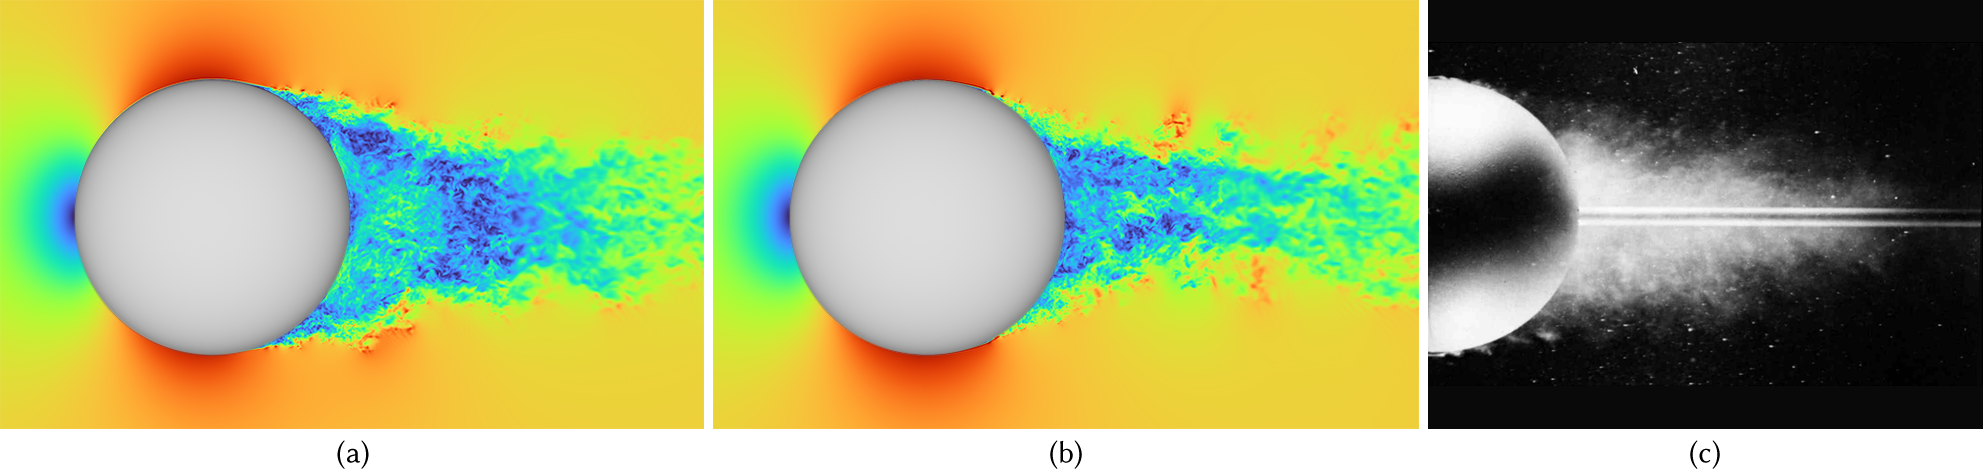
\includegraphics[width=0.99\columnwidth]{figures/wake_comp.png}
  \bicaption[球在发生阻力危机时的尾流]{球在发生阻力危机时的尾流。气流在$Re=400,000$下流过球时,由于固体边界附近的涡的尺度更小,尾流会收窄,从而阻力会下降。这一现象可见实际实验~\cite{Van-1982} (c)。与~\cite{Tao-2018-b} (a) 相比,在同样雷诺数下,我们的边界处理 (b) 捕捉到的边界的分离点更靠后,与实际实验更为接近。}{Wake of sphere in drag crisis. The flow passing through a sphere at $Re=400,000$ is known to exhibit in real-life experiment a narrower turbulent wake than at lower Reynolds numbers~\cite{Van-1982} (c) due to smaller scale vortices generated near the solid boundary, thus reducing drag significantly --- a paradox explained by the boundary-layer theory. Compared to~\cite{Tao-2018-b} (a), our improved boundary treatment scheme at the same Reynolds number (b) captures the separation point farther around the back of the sphere with a narrower wake, better matching the experimental visualization.}
  \label{img:sphere_wake_comp}
\end{figure}

\paragraph{与现有边界处理的对比}
为了验证我们的方法在边界处理上的精度提升,我们依然对雷诺数$Re=400,000$时,风流过球的阻力危机进行实验。如图~\ref{img:sphere_wake_comp} 所示,与实际实验的可视化相比 (图~\ref{img:sphere_wake_comp} (c)),我们的方法可以更好地预测固体边界附近的速度场及分离点 (图~\ref{img:sphere_wake_comp} (b))。并且,在图~\ref{img:bnd_comp} 中我们展示了不同方法得到的$C_\text{d}$与时间曲线,可见我们的方法得到的结果与真实实验最为匹配。这也说明在同样分辨率下,我们的方法与~\cite{Tao-2018-b} 相比,可以在固体边界上产生更小的涡流,使得尾流可以更加收敛,以在高雷诺数湍流仿真中获得更精准的结果。

\begin{figure}[!htbp]
\centering
  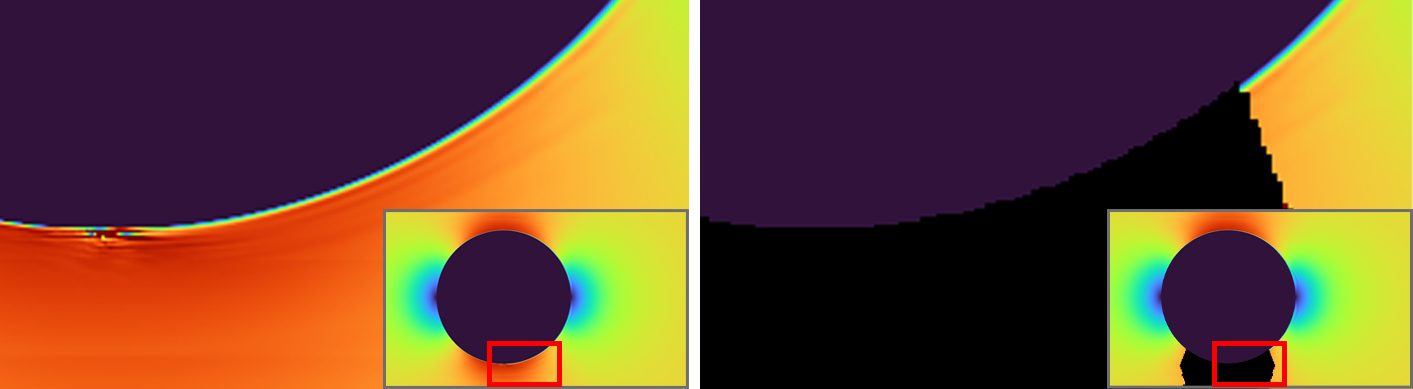
\includegraphics[width=0.99\columnwidth]{figures/wei_crash_vis.png}
\bicaption[图形学领域中最前沿的LBM方法的发散结果]{图形学领域中最前沿的LBM方法的发散结果。现有的图形学领域中的LBM方法都依赖于中心矩碰撞模型~\cite{Li-2020}。由于中心矩中的不同阶数的矩相对并不独立,且高阶松弛系数不一定准确,在使用多分辨率网格进行仿真时通常会得到发散结果,即使雷诺数并不足够高。这里展示了使用中心矩碰撞模型对$Re$=100,000时风吹过球的仿真结果。边界附近的速度求解错误 (左图) 最终导致整个求解结果发散 (右图中黑色区域)。}{Typical blowup of latest LBM solvers in CG. Existing LBM methods in CG mostly rely on central-moment collision models~\cite{Li-2020,Lyu:2021}. Due to the entangling of various orders of moments and improper high-order relaxation rates, they often blow up at low Reynolds numbers (here, $Re$=100,000) when simulating even a simple flow around the sphere with multiresolution grids, see black region (right), due to spurious velocities near the solid boundary (left).}
\label{img:wei_crash_vis}
\end{figure}

\paragraph{与图形学领域中LBM方法的对比}
虽然目前图形学领域中最前沿的LBM方法~\cite{Li-2020} 相比图形学领域中其它的流体仿真方法,已经显著地提升了精度与效率。但是对于工业领域的应用,这些方法在精度和稳定性上均有一定的差距。图~\ref{img:wei_crash_vis} 展示了一个使用图形学领域中的LBM方法进行的相对简单的气动仿真实验,即球在相对较低的雷诺数 ($Re$=100,000) 下的气动仿真。该仿真使用了与其它的球的气动仿真实验一致的多分辨率网格设置,但即使在分辨率相对较高的情况下,在仿真早期便开始出现不稳定现象,以至于数值发散而无法获得结果。

\section{方法的局限性}
我们的方法中也有一定的局限性。
首先,动态物体的精准处理在LBM中依然是一个待解决的问题,在我们的方法中,在静止场景求解时要比动态场景更加精准 (虽然这对于大部分流体求解方法也是类似的)。这一问题在第~\ref{sec:results_industry} 节的测试中有所体现。如何改进LBM的动态边界条件以获得更高的精度值得更深层的研究。
其次,在不规则网格中,我们采用的数据结构并没有足够的优化。这一问题在第~\ref{sec:sig23_alg_optimal} 中已有讨论,我们认为在这一方面也有一定的优化空间。
最后,LBM求解器与N-S求解器相比,通常需要更多的格点数与内存占用来达到相同的精度 (虽然LBM的效率要高得多)。如何减少LBM的内存消耗也是非常值得研究的方向。

\section{总结}
在本章中,我们提出了一个多分辨率的LBM流体仿真框架,以高效且准确地构建一个虚拟风洞测试系统,以评估模型的气动特性。
我们的方法基于现有CG与CFD领域中最先进的方法,在精度和效率上有所提升。这使得我们的方法可以不仅应用于视觉特效中的复杂流体仿真,也可以应用于如汽车、飞机、建筑等的设计、预览和评估,并通过快速的气动特性的反馈与分析,加速各个过程。

同时,我们的方法还弥合了CG与CFD领域中的方法差异。虽然CFD领域中不断在精度上对方法进行改进 (如更精准的碰撞模型与边界处理方法),但对求解器之外的一些重要方面,CFD领域甚少关注,如自动的多分辨率网格构建、高效的几何前处理与GPU实现等。这些在工业应用中也是十分关键的。而CG领域中,相比目前广泛使用的N-S求解器,通过使用我们的方法可以更简单、高效地完成湍流仿真与一些复杂的流体现象,这在之前的CG应用中是经常缺失的。

基于我们的工作,可以进行一些后续的工作。
首先,我们目前只处理了单向耦合,以处理虚拟风洞实验中最常见的场景。但增加对双向耦合的支持可以使我们的方法更加灵活,对实际工程与动画制作都有一定的应用价值。
此外,目前对于动态物体,我们的网格是不变的。支持动态的网格重构可以使内存使用进一步下降 (虽然可能会降低整体仿真效率)。
最后,构建一个虚拟的水下测试环境 (可以基于~\cite{Wei:2022, Wei:2023} 的工作) 以应对更复杂的场景也是一个极有意义但同时也极具挑战性的工作。